% -*- coding: UTF8 -*-
% \XeTeXinputencoding "UTF8"
\documentclass[a4paper,12pt]{examdesign}
\usepackage{tikz}
\usepackage{mathrsfs,pifont}
\usepackage{stmaryrd}
\usepackage{amsmath}
\usepackage[thinspace,thinqspace,squaren]{SIunits}
\usepackage[scale={.8,.8},footskip=12pt]{geometry}
\usepackage{lastpage,float}
\NumberOfVersions{1}
\usepackage[MnSymbol]{mathspec}
\usepackage[fullfamily,opticals,swash,minionint,openg,lf]{MinionPro}
\usepackage[PunctStyle=quanjiao]{xeCJK}
\setmainfont{Minion Pro}
\setsansfont{Myriad Pro}
% \setmonofont{FreeMono}
\setCJKmainfont[BoldFont={FZSongHei-B07S},
              ItalicFont={FZKaiTi},
              SlantedFont={FZFangSongTi}]{FZShuSong-Z01}
\setCJKsansfont[BoldFont={FZDaHei-B02S},
              ItalicFont={FZLiShu II-S06S},
              SlantedFont={FZCuYuan-M03S}]{FZHeiTi}
\setCJKmonofont[BoldFont={FZZhongDengXian-Z07S},
              ItalicFont={FZXiYuan-M01S},
              SlantedFont={FZBaoSong-Z04S}]{FZXiDengXian-Z06S}
\usepackage{graphicx}
%\usepackage{floatflt}
\newcommand{\chuhao}{\fontsize{42pt}{\baselineskip}\selectfont}
\newcommand{\xiaochuhao}{\fontsize{36pt}{\baselineskip}\selectfont}
\newcommand{\yihao}{\fontsize{28pt}{\baselineskip}\selectfont}
\newcommand{\erhao}{\fontsize{21pt}{\baselineskip}\selectfont}
\newcommand{\xiaoerhao}{\fontsize{18pt}{\baselineskip}\selectfont}
\newcommand{\sanhao}{\fontsize{15.75pt}{\baselineskip}\selectfont}
\newcommand{\sihao}{\fontsize{14pt}{\baselineskip}\selectfont}
\newcommand{\xiaosihao}{\fontsize{12pt}{\baselineskip}\selectfont}
\newcommand{\wuhao}{\fontsize{10.5pt}{\baselineskip}\selectfont}
\newcommand{\xiaowuhao}{\fontsize{9pt}{\baselineskip}\selectfont}
\newcommand{\liuhao}{\fontsize{7.875pt}{\baselineskip}\selectfont}
\newcommand{\qihao}{\fontsize{5.25pt}{\baselineskip}\selectfont}

\def\Varangle#1{\kern.75pt\vtop{\hbox{\kern-.75pt$/{#1}$}\kern-.35pt\hrule}}

\begin{document}
\DeclareGraphicsExtensions{.pdf}
\renewcommand\figurename{图}
\newcommand\AnswerLeading{解}
\SectionPrefix{}
% \NoKey
\NoRearrange
\ShortKey
\ProportionalBlanks{1.5}
\SectionFont{\large\bf}
\examname{电子测量}
\DefineAnswerWrapper{\begin{description}\item [\AnswerLeading:]}{\end{description}}
\def\namedata{\large学号\underline{\hspace{126pt}}姓名\underline{\hspace{98pt}}成绩\underline{\hspace{98pt}}}
\class{\large学院(部)\underline{\hspace{98pt}}年级\underline{\hspace{98pt}}专业\underline{\hspace{98pt}}}
\begin{examtop}
\setcounter{version}{2}
\begin{center}
\begin{tabular}{r}
    {\Large \bf 苏州大学
    \underline{\hspace{54pt}\examtype\hspace{54pt}} 课程}\hspace{9pt}\medskip \\
    {\Large \bf 期 \underline{\hspace{9pt}末\hspace{9pt}} 试卷
    \hspace{9pt}(\Alph{version}) 卷\hspace{36pt}共 4 页}\medskip\\
    {\large考试形式 \underline{\hspace{7pt}闭卷\hspace{7pt}}\hspace{48pt}2015 年 1 月}
\end{tabular}
\\\bigskip
\classdata\\ \namedata
\end{center}
\bigskip
\end{examtop}
\begin{keytop}
\begin{center}
\begin{tabular}{r}
    {\Large \bf 苏州大学
    \underline{\hspace{54pt}\examtype\hspace{54pt}} 课程}\hspace{9pt}\medskip \\
    {\Large \bf \hspace{17pt}期 \underline{\hspace{6pt}末\hspace{6pt}}
    试卷 (\Alph{version}) 卷\hspace{9pt}参考答案\hspace{12pt}共 \pageref{LastPage} 页}\medskip\\
    {\large考试形式 \underline{\hspace{7pt}闭卷\hspace{7pt}}\hspace{48pt}2015 年 1 月}
\end{tabular}
\end{center}
\bigskip
\end{keytop}

\newcommand\mathdot[1]{\dot#1}

\begin{fillin}[title={一、填空题 (每题 2 分,共 20 分)}]
    \begin{question}
        DVM 的固有测量误差通常用\blank{读数}误差和满度误差共同表示。
    \end{question}
    \begin{question}
        从广义上说,凡是利用\blank{电子技术}来进行的测量都可以说是电子测量。
    \end{question}
    \begin{question}
        锁相环是指由相位比较器、环路滤波器和\blank{压控振荡器}组成的闭合环路。
    \end{question}
    \begin{question}
        积分型数字电压表与比较型数字电压表相比具有\blank{抗干扰能力}强、但转换速度慢的特点。
    \end{question}
    \begin{question}
        电子计数器测周时是以\blank{被测信号}为闸门控制信号的。
    \end{question}
    \begin{question}
        计量工作的三个主要特征是\blank{统一性}、准确性和法制性。
    \end{question}
    \begin{question}
        电子计数器的测量周期时误差主要有量化误差,基准频率误差,\blank{
        触发转换}误差。
    \end{question}
    \begin{question}
        相对误差又叫相对真误差,它是\blank{绝对误差}与真值的比值。
    \end{question}
    \begin{question}
        交流电压峰值与有效值的比值称为\blank{波峰因数}。
    \end{question}
    \begin{question}
        在低频信号发生器中的主振级采用\blank{RC 振荡}电路。
    \end{question}
\end{fillin}

\begin{shortanswer}[title={二、计算题 (每题 10 分,共 80 分)}]

\begin{question}
    有一四位半数字电压表,基本量程为 \unit{2}{V},相邻量程间相差 10 倍,
    测量误差与被测电压读数 $U_x$ 的比例系数 $a\% = 0.03\%$,测量误差与测
    量所用量程 $U_\mathrm{m}$ 的比例系数 $b\% = 0.01\%$。求用该表测量约 \unit{0.5}{V} 电
    压时,应选用哪个量程,并求测量的相对误差范围。
    \examvspace*{3cm}
    \begin{answer}
        应选择 \unit{2}{V} 量程。$\gamma = \pm 0.07\%$。
    \end{answer}
\end{question}
\begin{question}
有一个固定频率的信号源,对其输出频率 $f$ 进行六次测量(可认为是独立、等精密度,无系统误差的测量),所得数据如下表: 
\begin{table}[H]
\centering
\begin{tabular}{|r|c|c|c|c|c|c|}
    \hline
    序号 i &1 &2 &3 &4 &5 &6 \\ \hline
    频率 $f_\mathrm{i}$ (kHz) &1001.032 &1001.501 &1001.199 &1002.011
    &1001.679 &1000.006 \\
    \hline
\end{tabular}
\end{table}
计算平均值 $\overline{f}$ 及标准偏差估计值 $s(f)$、$s(\overline{f})$。
    \examvspace*{9cm}
    \begin{answer}
        求频率 $f$ 的平均值 $\overline{f} = \unit{1001.238}{kHz}$。
        由贝塞尔公式求 $f$ 的标准偏差估计值 $s(f) = \unit{0.696}{kHz}$,
        求平均值的标准偏差估计值 $s(\overline{f}) = \unit{0.284}{kHz}$。
    \end{answer}
\end{question}
\begin{question}
某型电桥测量电容的技术指标如下:\\
范围:\unit{3}{pF} — \unit{11000}{\micro F}  共八档\\
最大允许误差:\\
\unit{100}{pF} 档:±(5\%指示值 + 0.5\%满度值) \\
\unit{1000}{pF} 档:±(3\%指示值 + 0.3\%满度值) \\
0.01、0.1、1、\unit{10}{\micro F} 各档:±(2\%指示值 + 0.3\%满度值) \\
\unit{100}{\micro F} 档:±(3\%指示值 + 0.3\%满度值) \\
\unit{1000}{\micro F} 档:±(5\%指示值 + 0.5\%满度值) \\
若用该电桥测量三个电容器,其指示值分别为 \unit{22}{pF},
\unit{0.33}{\micro F} 和 \unit{47}{\micro F},计算这些测量值的绝对误差和相对误差。
    \examvspace*{5cm}
    \begin{answer}
        (1) $\Delta C = 22 \times 5\% + 100 \times 0.5\% =
        \unit{1.6}{pF}$,$\gamma = 1.6/22 \times 100\% = 7.27\%$。\\
        (2) $\Delta C = 0.33 \times 2\%+1\times 0.3\% =
        \unit{0.0096}{\micro F}$,$\gamma = 0.0096/0.33 \times 100\% =
        2.91\%$。\\
        (3) $\Delta C = 47\times 3\%+100\times 0.3\% =
        \unit{1.71}{\micro F}$,$\gamma = 1.71/47 \times 100\% = 3.64\%$。
    \end{answer}
\end{question}
\begin{question}
    某计数器标准频率误差 $|\Delta f_\mathrm{C}/f_\mathrm{C}|=1\times
    10^{-9}$,利用该计数器将一个 \unit{20}{MHz} 的晶体振荡器校准到
    $10^{-7}$,则 (1) 计数器闸门时间应为多少?(2) 若要校准到 $10^{-9}$,则计数器闸门时间又应为多少?
    \examvspace*{5cm}
    \begin{answer}
        (1) 由频率误差 $\Delta f_x / f_x = 1/(Tf_x) + \Delta
        f_\mathrm{C}/f_\mathrm{C}$,要使 $|\Delta f_x/f_x| =
        10^{-7}$,则 $T \approx \unit{0.505}{\second}$。
        (2) 同理要使之达到 $10^{-9}$,则 $T=\infty$,即无法校准到
        $10^{-9}$。
    \end{answer}
\end{question}
\begin{question}
    利用正弦波有效值刻度的均值表测量正弦波、方波和三角波,读数均为
    \unit{1}{V},试求:(1) 正弦波信号的有效值;(2) 方波信号的有效值;(3) 三角波信号的有效值。
    \examvspace*{10cm}
    \begin{answer}
        (1) 正弦波,有效值 $U = \alpha = \unit{1}{V}$。
        (2) 方波,波形因数 1.0,平均值 $\overline{U} = \alpha / 1.11 =
        \unit{0.9}{V}$,有效值 $U = 1.0 \times \overline{U} =
        \unit{0.9}{V}$。
(3) 三角波,波形因数 1.15,平均值 $\overline{U} = \alpha / 1.11 =
        \unit{0.9}{V}$,有效值 $U = 1.15 \times \overline{U} =
        \unit{1.035}{V}$。
    \end{answer}
\end{question}
\begin{question}
    双积分式 DVM,基准电压 $U_\mathrm{r} = \unit{10}{V}$,设积分时间
    $T_1$ 时间计数值 $N_1 = 10000$, DVM 显示 $T_2$ 时间计数值 $N_2 =
    5600$,(1) 求被测电压 $U_x$;(2) 若要同时获得较好的工频抗干扰能力和
    较短的测量时间,时钟频率 $f_0$ 应取多少?
    \examvspace*{4cm}
    \begin{answer}
        (1) $U_x = N_2 U_\mathrm{r} / N_1 = \unit{5.6}{V}$。
   (2) 若要同时获得较好的工频抗干扰能力和较短的测量时间,$T_1$ 的时间应
   为工频周期的整数倍,取 5 倍,即 $T_1 = \unit{100}{ms}$,则 $f_0 = N_1
   / T_1 = \unit{100}{kHz}$。
    \end{answer}
\end{question}
\begin{question}
    一示波器的荧光屏的水平宽度为 \unit{10}{cm},现要求在上面最多显示
    \unit{1}{MHz} 正弦信号两个周期(幅度适当),问该示波器的扫描速度应该为多少?
    \examvspace*{4cm}
    \begin{answer}
        正弦信号频率为 \unit{1}{MHz},$T=\unit{1}{\micro s}$,要在屏幕
        上显示两个周期,则显示的时间为 $2T = \unit{2}{\micro s}$,扫描速
        度为 $S_\mathrm{S} = 2T / 10 = \unit{0.2}{\micro\second/cm}$。
    \end{answer}
\end{question}
\begin{question}
写出下图所示两个锁相环的输出频率 $f_o$ 的表达式。
    \begin{figure}[H]
        \centering
        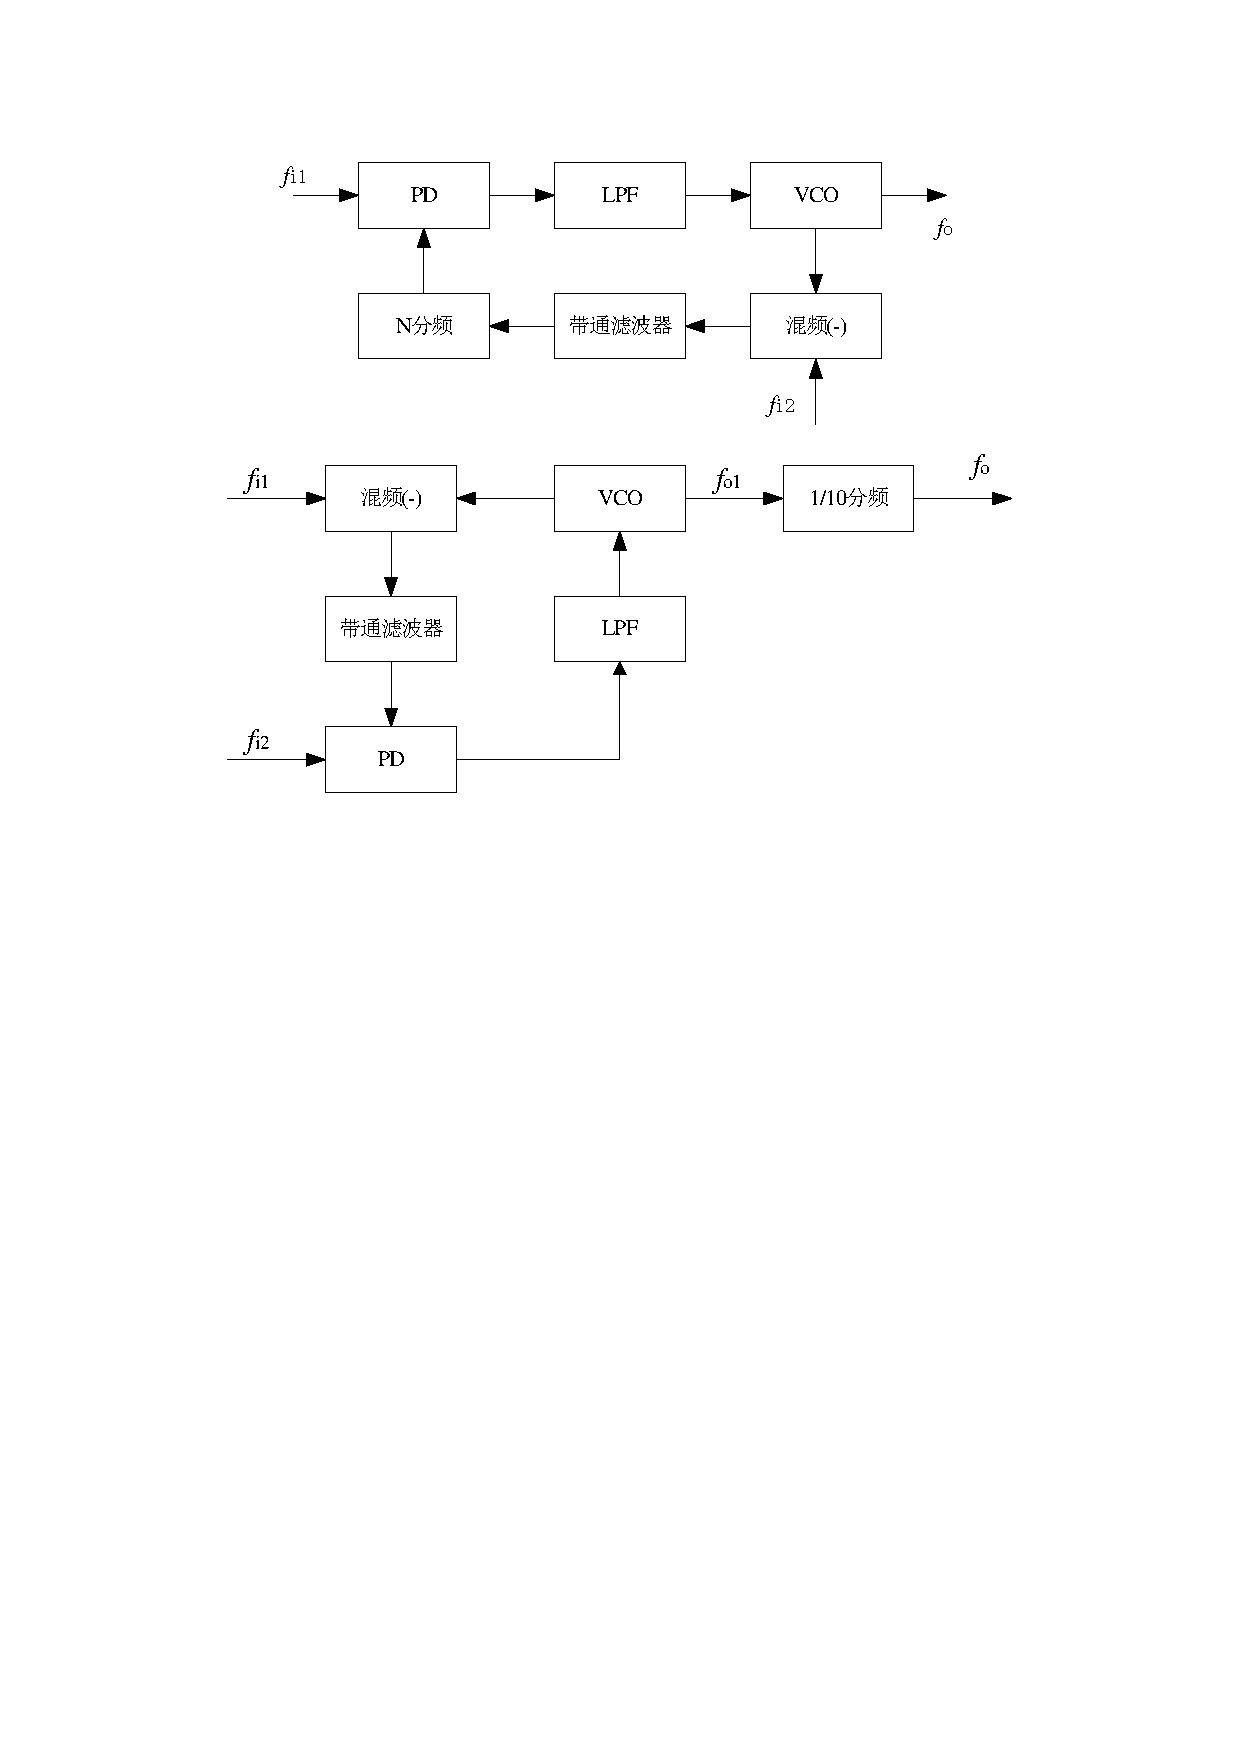
\includegraphics{pll}
    \end{figure}
    \examvspace*{0cm}
    \begin{answer}
        (1) $f_o = N\times f_{i1}+f_{i2}$。(2) $f_o = (f_{i1}+f_{i2})/10$。
    \end{answer}
\end{question}

\end{shortanswer}
\end{document}
